\documentclass[1p]{elsarticle_modified}
%\bibliographystyle{elsarticle-num}

%\usepackage[colorlinks]{hyperref}
%\usepackage{abbrmath_seonhwa} %\Abb, \Ascr, \Acal ,\Abf, \Afrak
\usepackage{amsfonts}
\usepackage{amssymb}
\usepackage{amsmath}
\usepackage{amsthm}
\usepackage{scalefnt}
\usepackage{amsbsy}
\usepackage{kotex}
\usepackage{caption}
\usepackage{subfig}
\usepackage{color}
\usepackage{graphicx}
\usepackage{xcolor} %% white, black, red, green, blue, cyan, magenta, yellow
\usepackage{float}
\usepackage{setspace}
\usepackage{hyperref}

\usepackage{tikz}
\usetikzlibrary{arrows}

\usepackage{multirow}
\usepackage{array} % fixed length table
\usepackage{hhline}

%%%%%%%%%%%%%%%%%%%%%
\makeatletter
\renewcommand*\env@matrix[1][\arraystretch]{%
	\edef\arraystretch{#1}%
	\hskip -\arraycolsep
	\let\@ifnextchar\new@ifnextchar
	\array{*\c@MaxMatrixCols c}}
\makeatother %https://tex.stackexchange.com/questions/14071/how-can-i-increase-the-line-spacing-in-a-matrix
%%%%%%%%%%%%%%%

\usepackage[normalem]{ulem}

\newcommand{\msout}[1]{\ifmmode\text{\sout{\ensuremath{#1}}}\else\sout{#1}\fi}
%SOURCE: \msout is \stkout macro in https://tex.stackexchange.com/questions/20609/strikeout-in-math-mode

\newcommand{\cancel}[1]{
	\ifmmode
	{\color{red}\msout{#1}}
	\else
	{\color{red}\sout{#1}}
	\fi
}

\newcommand{\add}[1]{
	{\color{blue}\uwave{#1}}
}

\newcommand{\replace}[2]{
	\ifmmode
	{\color{red}\msout{#1}}{\color{blue}\uwave{#2}}
	\else
	{\color{red}\sout{#1}}{\color{blue}\uwave{#2}}
	\fi
}

\newcommand{\Sol}{\mathcal{S}} %segment
\newcommand{\D}{D} %diagram
\newcommand{\A}{\mathcal{A}} %arc


%%%%%%%%%%%%%%%%%%%%%%%%%%%%%5 test

\def\sl{\operatorname{\textup{SL}}(2,\Cbb)}
\def\psl{\operatorname{\textup{PSL}}(2,\Cbb)}
\def\quan{\mkern 1mu \triangleright \mkern 1mu}

\theoremstyle{definition}
\newtheorem{thm}{Theorem}[section]
\newtheorem{prop}[thm]{Proposition}
\newtheorem{lem}[thm]{Lemma}
\newtheorem{ques}[thm]{Question}
\newtheorem{cor}[thm]{Corollary}
\newtheorem{defn}[thm]{Definition}
\newtheorem{exam}[thm]{Example}
\newtheorem{rmk}[thm]{Remark}
\newtheorem{alg}[thm]{Algorithm}

\newcommand{\I}{\sqrt{-1}}
\begin{document}

%\begin{frontmatter}
%
%\title{Boundary parabolic representations of knots up to 8 crossings}
%
%%% Group authors per affiliation:
%\author{Yunhi Cho} 
%\address{Department of Mathematics, University of Seoul, Seoul, Korea}
%\ead{yhcho@uos.ac.kr}
%
%
%\author{Seonhwa Kim} %\fnref{s_kim}}
%\address{Center for Geometry and Physics, Institute for Basic Science, Pohang, 37673, Korea}
%\ead{ryeona17@ibs.re.kr}
%
%\author{Hyuk Kim}
%\address{Department of Mathematical Sciences, Seoul National University, Seoul 08826, Korea}
%\ead{hyukkim@snu.ac.kr}
%
%\author{Seokbeom Yoon}
%\address{Department of Mathematical Sciences, Seoul National University, Seoul, 08826,  Korea}
%\ead{sbyoon15@snu.ac.kr}
%
%\begin{abstract}
%We find all boundary parabolic representation of knots up to 8 crossings.
%
%\end{abstract}
%\begin{keyword}
%    \MSC[2010] 57M25 
%\end{keyword}
%
%\end{frontmatter}

%\linenumbers
%\tableofcontents
%
\newcommand\colored[1]{\textcolor{white}{\rule[-0.35ex]{0.8em}{1.4ex}}\kern-0.8em\color{red} #1}%
%\newcommand\colored[1]{\textcolor{white}{ #1}\kern-2.17ex	\textcolor{white}{ #1}\kern-1.81ex	\textcolor{white}{ #1}\kern-2.15ex\color{red}#1	}

{\Large $\underline{12a_{0108}~(K12a_{0108})}$}

\setlength{\tabcolsep}{10pt}
\renewcommand{\arraystretch}{1.6}
\vspace{1cm}\begin{tabular}{m{100pt}>{\centering\arraybackslash}m{274pt}}
\multirow{5}{120pt}{
	\centering
	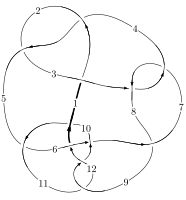
\includegraphics[width=112pt]{../../../GIT/diagram.site/Diagrams/png/909_12a_0108.png}\\
\ \ \ A knot diagram\footnotemark}&
\allowdisplaybreaks
\textbf{Linearized knot diagam} \\
\cline{2-2}
 &
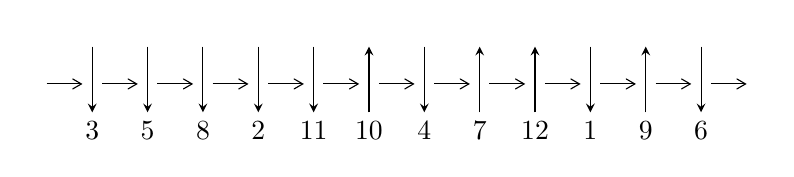
\begin{tikzpicture}[x=20pt, y=17pt]
	% nodes
	\node (C0) at (0, 0) {};
	\node (C1) at (1, 0) {};
	\node (C1U) at (1, +1) {};
	\node (C1D) at (1, -1) {3};

	\node (C2) at (2, 0) {};
	\node (C2U) at (2, +1) {};
	\node (C2D) at (2, -1) {5};

	\node (C3) at (3, 0) {};
	\node (C3U) at (3, +1) {};
	\node (C3D) at (3, -1) {8};

	\node (C4) at (4, 0) {};
	\node (C4U) at (4, +1) {};
	\node (C4D) at (4, -1) {2};

	\node (C5) at (5, 0) {};
	\node (C5U) at (5, +1) {};
	\node (C5D) at (5, -1) {11};

	\node (C6) at (6, 0) {};
	\node (C6U) at (6, +1) {};
	\node (C6D) at (6, -1) {10};

	\node (C7) at (7, 0) {};
	\node (C7U) at (7, +1) {};
	\node (C7D) at (7, -1) {4};

	\node (C8) at (8, 0) {};
	\node (C8U) at (8, +1) {};
	\node (C8D) at (8, -1) {7};

	\node (C9) at (9, 0) {};
	\node (C9U) at (9, +1) {};
	\node (C9D) at (9, -1) {12};

	\node (C10) at (10, 0) {};
	\node (C10U) at (10, +1) {};
	\node (C10D) at (10, -1) {1};

	\node (C11) at (11, 0) {};
	\node (C11U) at (11, +1) {};
	\node (C11D) at (11, -1) {9};

	\node (C12) at (12, 0) {};
	\node (C12U) at (12, +1) {};
	\node (C12D) at (12, -1) {6};
	\node (C13) at (13, 0) {};

	% arrows
	\draw[->,>={angle 60}]
	(C0) edge (C1) (C1) edge (C2) (C2) edge (C3) (C3) edge (C4) (C4) edge (C5) (C5) edge (C6) (C6) edge (C7) (C7) edge (C8) (C8) edge (C9) (C9) edge (C10) (C10) edge (C11) (C11) edge (C12) (C12) edge (C13) ;	\draw[->,>=stealth]
	(C1U) edge (C1D) (C2U) edge (C2D) (C3U) edge (C3D) (C4U) edge (C4D) (C5U) edge (C5D) (C6D) edge (C6U) (C7U) edge (C7D) (C8D) edge (C8U) (C9D) edge (C9U) (C10U) edge (C10D) (C11D) edge (C11U) (C12U) edge (C12D) ;
	\end{tikzpicture} \\
\hhline{~~} \\& 
\textbf{Solving Sequence} \\ \cline{2-2} 
 &
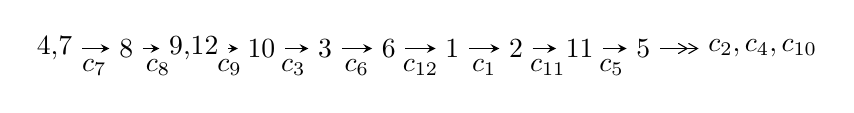
\begin{tikzpicture}[x=23pt, y=7pt]
	% node
	\node (A0) at (-1/8, 0) {4,7};
	\node (A1) at (1, 0) {8};
	\node (A2) at (33/16, 0) {9,12};
	\node (A3) at (25/8, 0) {10};
	\node (A4) at (33/8, 0) {3};
	\node (A5) at (41/8, 0) {6};
	\node (A6) at (49/8, 0) {1};
	\node (A7) at (57/8, 0) {2};
	\node (A8) at (65/8, 0) {11};
	\node (A9) at (73/8, 0) {5};
	\node (C1) at (1/2, -1) {$c_{7}$};
	\node (C2) at (3/2, -1) {$c_{8}$};
	\node (C3) at (21/8, -1) {$c_{9}$};
	\node (C4) at (29/8, -1) {$c_{3}$};
	\node (C5) at (37/8, -1) {$c_{6}$};
	\node (C6) at (45/8, -1) {$c_{12}$};
	\node (C7) at (53/8, -1) {$c_{1}$};
	\node (C8) at (61/8, -1) {$c_{11}$};
	\node (C9) at (69/8, -1) {$c_{5}$};
	\node (A10) at (11, 0) {$c_{2},c_{4},c_{10}$};

	% edge
	\draw[->,>=stealth]	
	(A0) edge (A1) (A1) edge (A2) (A2) edge (A3) (A3) edge (A4) (A4) edge (A5) (A5) edge (A6) (A6) edge (A7) (A7) edge (A8) (A8) edge (A9) ;
	\draw[->>,>={angle 60}]	
	(A9) edge (A10);
\end{tikzpicture} \\ 

\end{tabular} \\

\footnotetext{
The image of knot diagram is generated by the software ``\textbf{Draw programme}" developed by Andrew Bartholomew(\url{http://www.layer8.co.uk/maths/draw/index.htm\#Running-draw}), where we modified some parts for our purpose(\url{https://github.com/CATsTAILs/LinksPainter}).
}\phantom \\ \newline 
\centering \textbf{Ideals for irreducible components\footnotemark of $X_{\text{par}}$} 
 
\begin{align*}
I^u_{1}&=\langle 
-7.77659\times10^{312} u^{125}-1.54560\times10^{313} u^{124}+\cdots+7.56628\times10^{313} b-1.03264\times10^{314},\\
\phantom{I^u_{1}}&\phantom{= \langle  }-1.29367\times10^{314} u^{125}-2.52409\times10^{314} u^{124}+\cdots+1.66458\times10^{315} a+2.23551\times10^{316},\\
\phantom{I^u_{1}}&\phantom{= \langle  }u^{126}+2 u^{125}+\cdots+192 u+64\rangle \\
I^u_{2}&=\langle 
3 u^2+b+u+3,\;6 u^2+a+2 u+10,\;u^3+u^2+2 u+1\rangle \\
\\
I^v_{1}&=\langle 
a,\;31 v^5-92 v^4+163 v^3+52 v^2+69 b+81 v-64,\;v^6-3 v^5+6 v^4+5 v^2- v+1\rangle \\
\end{align*}
\raggedright * 3 irreducible components of $\dim_{\mathbb{C}}=0$, with total 135 representations.\\
\footnotetext{All coefficients of polynomials are rational numbers. But the coefficients are sometimes approximated in decimal forms when there is not enough margin.}
\newpage
\renewcommand{\arraystretch}{1}
\centering \section*{I. $I^u_{1}= \langle -7.78\times10^{312} u^{125}-1.55\times10^{313} u^{124}+\cdots+7.57\times10^{313} b-1.03\times10^{314},\;-1.29\times10^{314} u^{125}-2.52\times10^{314} u^{124}+\cdots+1.66\times10^{315} a+2.24\times10^{316},\;u^{126}+2 u^{125}+\cdots+192 u+64 \rangle$}
\flushleft \textbf{(i) Arc colorings}\\
\begin{tabular}{m{7pt} m{180pt} m{7pt} m{180pt} }
\flushright $a_{4}=$&$\begin{pmatrix}0\\u\end{pmatrix}$ \\
\flushright $a_{7}=$&$\begin{pmatrix}1\\0\end{pmatrix}$ \\
\flushright $a_{8}=$&$\begin{pmatrix}1\\u^2\end{pmatrix}$ \\
\flushright $a_{9}=$&$\begin{pmatrix}u^2+1\\u^2\end{pmatrix}$ \\
\flushright $a_{12}=$&$\begin{pmatrix}0.0777175 u^{125}+0.151635 u^{124}+\cdots-12.0430 u-13.4298\\0.102780 u^{125}+0.204274 u^{124}+\cdots+21.2752 u+1.36479\end{pmatrix}$ \\
\flushright $a_{10}=$&$\begin{pmatrix}-0.251458 u^{125}-0.504776 u^{124}+\cdots-62.6343 u-15.8172\\-0.125368 u^{125}-0.296640 u^{124}+\cdots-55.2984 u-10.6403\end{pmatrix}$ \\
\flushright $a_{3}=$&$\begin{pmatrix}u\\u^3+u\end{pmatrix}$ \\
\flushright $a_{6}=$&$\begin{pmatrix}0.184749 u^{125}+0.229941 u^{124}+\cdots+26.0397 u-4.61527\\0.128633 u^{125}+0.222528 u^{124}+\cdots+38.3890 u+5.67195\end{pmatrix}$ \\
\flushright $a_{1}=$&$\begin{pmatrix}0.134423 u^{125}+0.249675 u^{124}+\cdots-15.7540 u-12.1955\\-0.0161903 u^{125}-0.0611574 u^{124}+\cdots-50.9747 u-14.3007\end{pmatrix}$ \\
\flushright $a_{2}=$&$\begin{pmatrix}0.116123 u^{125}+0.204715 u^{124}+\cdots-22.9544 u-12.7987\\-0.0366348 u^{125}-0.0898334 u^{124}+\cdots-55.3988 u-14.3689\end{pmatrix}$ \\
\flushright $a_{11}=$&$\begin{pmatrix}0.0236074 u^{125}+0.0498670 u^{124}+\cdots-20.2156 u-13.1289\\0.150252 u^{125}+0.329184 u^{124}+\cdots+32.2910 u+2.86962\end{pmatrix}$ \\
\flushright $a_{5}=$&$\begin{pmatrix}0.0842320 u^{125}+0.177889 u^{124}+\cdots+30.2985 u+3.33220\\-0.0501911 u^{125}-0.0717859 u^{124}+\cdots+46.0525 u+15.5277\end{pmatrix}$\\&\end{tabular}
\flushleft \textbf{(ii) Obstruction class $= -1$}\\~\\
\flushleft \textbf{(iii) Cusp Shapes $= -0.597782 u^{125}-0.910341 u^{124}+\cdots-72.2510 u+19.0666$}\\~\\
\newpage\renewcommand{\arraystretch}{1}
\flushleft \textbf{(iv) u-Polynomials at the component}\newline \\
\begin{tabular}{m{50pt}|m{274pt}}
Crossings & \hspace{64pt}u-Polynomials at each crossing \\
\hline $$\begin{aligned}c_{1}\end{aligned}$$&$\begin{aligned}
&u^{126}+68 u^{125}+\cdots-17 u+1
\end{aligned}$\\
\hline $$\begin{aligned}c_{2},c_{4}\end{aligned}$$&$\begin{aligned}
&u^{126}-8 u^{125}+\cdots-9 u+1
\end{aligned}$\\
\hline $$\begin{aligned}c_{3},c_{7}\end{aligned}$$&$\begin{aligned}
&u^{126}+2 u^{125}+\cdots+192 u+64
\end{aligned}$\\
\hline $$\begin{aligned}c_{5}\end{aligned}$$&$\begin{aligned}
&u^{126}-65 u^{124}+\cdots+4405 u-191
\end{aligned}$\\
\hline $$\begin{aligned}c_{6}\end{aligned}$$&$\begin{aligned}
&u^{126}+4 u^{125}+\cdots-1174 u-44
\end{aligned}$\\
\hline $$\begin{aligned}c_{8}\end{aligned}$$&$\begin{aligned}
&u^{126}-42 u^{125}+\cdots-118784 u+4096
\end{aligned}$\\
\hline $$\begin{aligned}c_{9},c_{11}\end{aligned}$$&$\begin{aligned}
&u^{126}+5 u^{125}+\cdots-43 u-1
\end{aligned}$\\
\hline $$\begin{aligned}c_{10}\end{aligned}$$&$\begin{aligned}
&u^{126}-20 u^{125}+\cdots+124 u+8
\end{aligned}$\\
\hline $$\begin{aligned}c_{12}\end{aligned}$$&$\begin{aligned}
&u^{126}-9 u^{125}+\cdots+2 u-1
\end{aligned}$\\
\hline
\end{tabular}\\~\\
\newpage\renewcommand{\arraystretch}{1}
\flushleft \textbf{(v) Riley Polynomials at the component}\newline \\
\begin{tabular}{m{50pt}|m{274pt}}
Crossings & \hspace{64pt}Riley Polynomials at each crossing \\
\hline $$\begin{aligned}c_{1}\end{aligned}$$&$\begin{aligned}
&y^{126}-12 y^{125}+\cdots-363 y+1
\end{aligned}$\\
\hline $$\begin{aligned}c_{2},c_{4}\end{aligned}$$&$\begin{aligned}
&y^{126}-68 y^{125}+\cdots+17 y+1
\end{aligned}$\\
\hline $$\begin{aligned}c_{3},c_{7}\end{aligned}$$&$\begin{aligned}
&y^{126}+42 y^{125}+\cdots+118784 y+4096
\end{aligned}$\\
\hline $$\begin{aligned}c_{5}\end{aligned}$$&$\begin{aligned}
&y^{126}-130 y^{125}+\cdots-3185069 y+36481
\end{aligned}$\\
\hline $$\begin{aligned}c_{6}\end{aligned}$$&$\begin{aligned}
&y^{126}-122 y^{125}+\cdots-141964 y+1936
\end{aligned}$\\
\hline $$\begin{aligned}c_{8}\end{aligned}$$&$\begin{aligned}
&y^{126}+74 y^{125}+\cdots-125829120 y+16777216
\end{aligned}$\\
\hline $$\begin{aligned}c_{9},c_{11}\end{aligned}$$&$\begin{aligned}
&y^{126}-75 y^{125}+\cdots-971 y+1
\end{aligned}$\\
\hline $$\begin{aligned}c_{10}\end{aligned}$$&$\begin{aligned}
&y^{126}-24 y^{125}+\cdots-8848 y+64
\end{aligned}$\\
\hline $$\begin{aligned}c_{12}\end{aligned}$$&$\begin{aligned}
&y^{126}+15 y^{125}+\cdots-14 y+1
\end{aligned}$\\
\hline
\end{tabular}\\~\\
\newpage\flushleft \textbf{(vi) Complex Volumes and Cusp Shapes}
$$\begin{array}{c|c|c}  
\text{Solutions to }I^u_{1}& \I (\text{vol} + \sqrt{-1}CS) & \text{Cusp shape}\\
 \hline 
\begin{aligned}
u &= -0.583149 + 0.813259 I \\
a &= -2.40429 - 0.88467 I \\
b &= -2.36089 + 0.71738 I\end{aligned}
 & \phantom{-}0.84437 + 1.77385 I & \phantom{-0.000000 } 0 \\ \hline\begin{aligned}
u &= -0.583149 - 0.813259 I \\
a &= -2.40429 + 0.88467 I \\
b &= -2.36089 - 0.71738 I\end{aligned}
 & \phantom{-}0.84437 - 1.77385 I & \phantom{-0.000000 } 0 \\ \hline\begin{aligned}
u &= \phantom{-}0.759752 + 0.658456 I \\
a &= \phantom{-}0.411118 + 0.209764 I \\
b &= -0.228083 - 0.339879 I\end{aligned}
 & -3.19646 + 2.28892 I & \phantom{-0.000000 } 0 \\ \hline\begin{aligned}
u &= \phantom{-}0.759752 - 0.658456 I \\
a &= \phantom{-}0.411118 - 0.209764 I \\
b &= -0.228083 + 0.339879 I\end{aligned}
 & -3.19646 - 2.28892 I & \phantom{-0.000000 } 0 \\ \hline\begin{aligned}
u &= -0.664545 + 0.755167 I \\
a &= -0.12102 + 2.46179 I \\
b &= \phantom{-}1.225020 + 0.310188 I\end{aligned}
 & -1.33049 + 2.05219 I & \phantom{-0.000000 } 0 \\ \hline\begin{aligned}
u &= -0.664545 - 0.755167 I \\
a &= -0.12102 - 2.46179 I \\
b &= \phantom{-}1.225020 - 0.310188 I\end{aligned}
 & -1.33049 - 2.05219 I & \phantom{-0.000000 } 0 \\ \hline\begin{aligned}
u &= \phantom{-}0.638089 + 0.779199 I \\
a &= \phantom{-}1.54419 + 1.11191 I \\
b &= \phantom{-}0.88077 + 1.29949 I\end{aligned}
 & -5.12052 - 2.76244 I & \phantom{-0.000000 } 0 \\ \hline\begin{aligned}
u &= \phantom{-}0.638089 - 0.779199 I \\
a &= \phantom{-}1.54419 - 1.11191 I \\
b &= \phantom{-}0.88077 - 1.29949 I\end{aligned}
 & -5.12052 + 2.76244 I & \phantom{-0.000000 } 0 \\ \hline\begin{aligned}
u &= \phantom{-}1.008890 + 0.070007 I \\
a &= \phantom{-}2.21899 + 0.03163 I \\
b &= \phantom{-}1.73462 + 0.26110 I\end{aligned}
 & \phantom{-}2.18854 + 7.22641 I & \phantom{-0.000000 } 0 \\ \hline\begin{aligned}
u &= \phantom{-}1.008890 - 0.070007 I \\
a &= \phantom{-}2.21899 - 0.03163 I \\
b &= \phantom{-}1.73462 - 0.26110 I\end{aligned}
 & \phantom{-}2.18854 - 7.22641 I & \phantom{-0.000000 } 0\\
 \hline 
 \end{array}$$\newpage$$\begin{array}{c|c|c}  
\text{Solutions to }I^u_{1}& \I (\text{vol} + \sqrt{-1}CS) & \text{Cusp shape}\\
 \hline 
\begin{aligned}
u &= -0.134506 + 1.012070 I \\
a &= -0.72834 + 1.25076 I \\
b &= \phantom{-}4.00557 + 0.08173 I\end{aligned}
 & \phantom{-}3.77115 + 2.20092 I & \phantom{-0.000000 } 0 \\ \hline\begin{aligned}
u &= -0.134506 - 1.012070 I \\
a &= -0.72834 - 1.25076 I \\
b &= \phantom{-}4.00557 - 0.08173 I\end{aligned}
 & \phantom{-}3.77115 - 2.20092 I & \phantom{-0.000000 } 0 \\ \hline\begin{aligned}
u &= -0.236806 + 0.993858 I \\
a &= \phantom{-}0.049581 - 0.414116 I \\
b &= -0.407535 - 0.842117 I\end{aligned}
 & \phantom{-}1.90248 + 2.83956 I & \phantom{-0.000000 } 0 \\ \hline\begin{aligned}
u &= -0.236806 - 0.993858 I \\
a &= \phantom{-}0.049581 + 0.414116 I \\
b &= -0.407535 + 0.842117 I\end{aligned}
 & \phantom{-}1.90248 - 2.83956 I & \phantom{-0.000000 } 0 \\ \hline\begin{aligned}
u &= -0.077039 + 1.019420 I \\
a &= -0.395957 - 0.895205 I \\
b &= -0.345162 - 0.284694 I\end{aligned}
 & \phantom{-}2.60094 + 2.12761 I & \phantom{-0.000000 } 0 \\ \hline\begin{aligned}
u &= -0.077039 - 1.019420 I \\
a &= -0.395957 + 0.895205 I \\
b &= -0.345162 + 0.284694 I\end{aligned}
 & \phantom{-}2.60094 - 2.12761 I & \phantom{-0.000000 } 0 \\ \hline\begin{aligned}
u &= -0.870239 + 0.437016 I \\
a &= \phantom{-}2.01350 - 0.73003 I \\
b &= \phantom{-}1.27645 - 0.83997 I\end{aligned}
 & -1.62685 - 0.40405 I & \phantom{-0.000000 } 0 \\ \hline\begin{aligned}
u &= -0.870239 - 0.437016 I \\
a &= \phantom{-}2.01350 + 0.73003 I \\
b &= \phantom{-}1.27645 + 0.83997 I\end{aligned}
 & -1.62685 + 0.40405 I & \phantom{-0.000000 } 0 \\ \hline\begin{aligned}
u &= -0.750514 + 0.607886 I \\
a &= -0.48073 + 2.04336 I \\
b &= -0.174005 + 0.510313 I\end{aligned}
 & \phantom{-}0.258302 - 1.180800 I & \phantom{-0.000000 } 0 \\ \hline\begin{aligned}
u &= -0.750514 - 0.607886 I \\
a &= -0.48073 - 2.04336 I \\
b &= -0.174005 - 0.510313 I\end{aligned}
 & \phantom{-}0.258302 + 1.180800 I & \phantom{-0.000000 } 0\\
 \hline 
 \end{array}$$\newpage$$\begin{array}{c|c|c}  
\text{Solutions to }I^u_{1}& \I (\text{vol} + \sqrt{-1}CS) & \text{Cusp shape}\\
 \hline 
\begin{aligned}
u &= -0.701966 + 0.759826 I \\
a &= \phantom{-}1.88316 - 0.88061 I \\
b &= \phantom{-}1.45456 - 1.13212 I\end{aligned}
 & -3.74921 - 4.56977 I & \phantom{-0.000000 } 0 \\ \hline\begin{aligned}
u &= -0.701966 - 0.759826 I \\
a &= \phantom{-}1.88316 + 0.88061 I \\
b &= \phantom{-}1.45456 + 1.13212 I\end{aligned}
 & -3.74921 + 4.56977 I & \phantom{-0.000000 } 0 \\ \hline\begin{aligned}
u &= \phantom{-}0.745954 + 0.737217 I \\
a &= \phantom{-}2.05866 - 4.11011 I \\
b &= \phantom{-}2.80767 - 0.70209 I\end{aligned}
 & -2.73974 + 0.70736 I & \phantom{-0.000000 } 0 \\ \hline\begin{aligned}
u &= \phantom{-}0.745954 - 0.737217 I \\
a &= \phantom{-}2.05866 + 4.11011 I \\
b &= \phantom{-}2.80767 + 0.70209 I\end{aligned}
 & -2.73974 - 0.70736 I & \phantom{-0.000000 } 0 \\ \hline\begin{aligned}
u &= -0.089485 + 0.946069 I \\
a &= \phantom{-}1.28925 - 1.00533 I \\
b &= -1.55692 + 0.09969 I\end{aligned}
 & \phantom{-}0.43085 - 5.09047 I & \phantom{-0.000000 } 0 \\ \hline\begin{aligned}
u &= -0.089485 - 0.946069 I \\
a &= \phantom{-}1.28925 + 1.00533 I \\
b &= -1.55692 - 0.09969 I\end{aligned}
 & \phantom{-}0.43085 + 5.09047 I & \phantom{-0.000000 } 0 \\ \hline\begin{aligned}
u &= -0.026963 + 0.943464 I \\
a &= -0.404065 + 0.007320 I \\
b &= -0.922484 + 0.758848 I\end{aligned}
 & \phantom{-}2.41442 + 1.40190 I & \phantom{-0.000000 } 0 \\ \hline\begin{aligned}
u &= -0.026963 - 0.943464 I \\
a &= -0.404065 - 0.007320 I \\
b &= -0.922484 - 0.758848 I\end{aligned}
 & \phantom{-}2.41442 - 1.40190 I & \phantom{-0.000000 } 0 \\ \hline\begin{aligned}
u &= -1.036680 + 0.220066 I \\
a &= \phantom{-}2.08600 - 0.38383 I \\
b &= \phantom{-}1.56493 - 0.14601 I\end{aligned}
 & \phantom{-}1.84155 + 2.77321 I & \phantom{-0.000000 } 0 \\ \hline\begin{aligned}
u &= -1.036680 - 0.220066 I \\
a &= \phantom{-}2.08600 + 0.38383 I \\
b &= \phantom{-}1.56493 + 0.14601 I\end{aligned}
 & \phantom{-}1.84155 - 2.77321 I & \phantom{-0.000000 } 0\\
 \hline 
 \end{array}$$\newpage$$\begin{array}{c|c|c}  
\text{Solutions to }I^u_{1}& \I (\text{vol} + \sqrt{-1}CS) & \text{Cusp shape}\\
 \hline 
\begin{aligned}
u &= \phantom{-}0.902790 + 0.575810 I \\
a &= \phantom{-}2.16135 + 0.69093 I \\
b &= \phantom{-}1.72111 + 0.92699 I\end{aligned}
 & \phantom{-}0.07212 + 8.10921 I & \phantom{-0.000000 } 0 \\ \hline\begin{aligned}
u &= \phantom{-}0.902790 - 0.575810 I \\
a &= \phantom{-}2.16135 - 0.69093 I \\
b &= \phantom{-}1.72111 - 0.92699 I\end{aligned}
 & \phantom{-}0.07212 - 8.10921 I & \phantom{-0.000000 } 0 \\ \hline\begin{aligned}
u &= \phantom{-}0.515649 + 0.940162 I \\
a &= -0.80683 - 1.94203 I \\
b &= \phantom{-}0.490259 - 0.645229 I\end{aligned}
 & \phantom{-}4.07539 - 1.91046 I & \phantom{-0.000000 } 0 \\ \hline\begin{aligned}
u &= \phantom{-}0.515649 - 0.940162 I \\
a &= -0.80683 + 1.94203 I \\
b &= \phantom{-}0.490259 + 0.645229 I\end{aligned}
 & \phantom{-}4.07539 + 1.91046 I & \phantom{-0.000000 } 0 \\ \hline\begin{aligned}
u &= \phantom{-}0.821210 + 0.696105 I \\
a &= -3.79378 + 1.02212 I \\
b &= -3.05665 - 0.68146 I\end{aligned}
 & -2.64594 + 1.92186 I & \phantom{-0.000000 } 0 \\ \hline\begin{aligned}
u &= \phantom{-}0.821210 - 0.696105 I \\
a &= -3.79378 - 1.02212 I \\
b &= -3.05665 + 0.68146 I\end{aligned}
 & -2.64594 - 1.92186 I & \phantom{-0.000000 } 0 \\ \hline\begin{aligned}
u &= \phantom{-}0.066247 + 1.075380 I \\
a &= -1.104920 - 0.720837 I \\
b &= \phantom{-}1.083610 - 0.383367 I\end{aligned}
 & \phantom{-}6.12098 - 0.47562 I & \phantom{-0.000000 } 0 \\ \hline\begin{aligned}
u &= \phantom{-}0.066247 - 1.075380 I \\
a &= -1.104920 + 0.720837 I \\
b &= \phantom{-}1.083610 + 0.383367 I\end{aligned}
 & \phantom{-}6.12098 + 0.47562 I & \phantom{-0.000000 } 0 \\ \hline\begin{aligned}
u &= -0.866742 + 0.650126 I \\
a &= -0.929827 + 0.051878 I \\
b &= -1.310250 + 0.281104 I\end{aligned}
 & -1.08056 - 4.64409 I & \phantom{-0.000000 } 0 \\ \hline\begin{aligned}
u &= -0.866742 - 0.650126 I \\
a &= -0.929827 - 0.051878 I \\
b &= -1.310250 - 0.281104 I\end{aligned}
 & -1.08056 + 4.64409 I & \phantom{-0.000000 } 0\\
 \hline 
 \end{array}$$\newpage$$\begin{array}{c|c|c}  
\text{Solutions to }I^u_{1}& \I (\text{vol} + \sqrt{-1}CS) & \text{Cusp shape}\\
 \hline 
\begin{aligned}
u &= \phantom{-}0.164623 + 1.090970 I \\
a &= -0.937838 - 0.153506 I \\
b &= \phantom{-}1.274750 + 0.205009 I\end{aligned}
 & \phantom{-}5.90160 - 4.26455 I & \phantom{-0.000000 } 0 \\ \hline\begin{aligned}
u &= \phantom{-}0.164623 - 1.090970 I \\
a &= -0.937838 + 0.153506 I \\
b &= \phantom{-}1.274750 - 0.205009 I\end{aligned}
 & \phantom{-}5.90160 + 4.26455 I & \phantom{-0.000000 } 0 \\ \hline\begin{aligned}
u &= -0.612029 + 0.921384 I \\
a &= \phantom{-}1.39754 + 3.67655 I \\
b &= \phantom{-}3.36533 + 0.62198 I\end{aligned}
 & \phantom{-}1.22072 + 2.96447 I & \phantom{-0.000000 } 0 \\ \hline\begin{aligned}
u &= -0.612029 - 0.921384 I \\
a &= \phantom{-}1.39754 - 3.67655 I \\
b &= \phantom{-}3.36533 - 0.62198 I\end{aligned}
 & \phantom{-}1.22072 - 2.96447 I & \phantom{-0.000000 } 0 \\ \hline\begin{aligned}
u &= \phantom{-}0.608068 + 0.939760 I \\
a &= \phantom{-}0.48099 + 2.26771 I \\
b &= -1.36323 + 1.12639 I\end{aligned}
 & -4.61530 - 2.13294 I & \phantom{-0.000000 } 0 \\ \hline\begin{aligned}
u &= \phantom{-}0.608068 - 0.939760 I \\
a &= \phantom{-}0.48099 - 2.26771 I \\
b &= -1.36323 - 1.12639 I\end{aligned}
 & -4.61530 + 2.13294 I & \phantom{-0.000000 } 0 \\ \hline\begin{aligned}
u &= -0.715251 + 0.862634 I \\
a &= -0.756830 + 0.170735 I \\
b &= \phantom{-}0.355188 + 0.261563 I\end{aligned}
 & -6.56601 + 3.77378 I & \phantom{-0.000000 } 0 \\ \hline\begin{aligned}
u &= -0.715251 - 0.862634 I \\
a &= -0.756830 - 0.170735 I \\
b &= \phantom{-}0.355188 - 0.261563 I\end{aligned}
 & -6.56601 - 3.77378 I & \phantom{-0.000000 } 0 \\ \hline\begin{aligned}
u &= -0.712315 + 0.865143 I \\
a &= \phantom{-}0.170620 + 0.028930 I \\
b &= -0.416168 + 0.527299 I\end{aligned}
 & -6.55718 + 1.68165 I & \phantom{-0.000000 } 0 \\ \hline\begin{aligned}
u &= -0.712315 - 0.865143 I \\
a &= \phantom{-}0.170620 - 0.028930 I \\
b &= -0.416168 - 0.527299 I\end{aligned}
 & -6.55718 - 1.68165 I & \phantom{-0.000000 } 0\\
 \hline 
 \end{array}$$\newpage$$\begin{array}{c|c|c}  
\text{Solutions to }I^u_{1}& \I (\text{vol} + \sqrt{-1}CS) & \text{Cusp shape}\\
 \hline 
\begin{aligned}
u &= \phantom{-}0.283809 + 1.084470 I \\
a &= -0.430557 + 0.774152 I \\
b &= -0.040161 + 0.255290 I\end{aligned}
 & \phantom{-}1.79448 - 6.78921 I & \phantom{-0.000000 } 0 \\ \hline\begin{aligned}
u &= \phantom{-}0.283809 - 1.084470 I \\
a &= -0.430557 - 0.774152 I \\
b &= -0.040161 - 0.255290 I\end{aligned}
 & \phantom{-}1.79448 + 6.78921 I & \phantom{-0.000000 } 0 \\ \hline\begin{aligned}
u &= -0.837606 + 0.789777 I \\
a &= \phantom{-}0.715847 - 0.779366 I \\
b &= \phantom{-}0.193028 - 0.396166 I\end{aligned}
 & -1.93800 + 2.88339 I & \phantom{-0.000000 } 0 \\ \hline\begin{aligned}
u &= -0.837606 - 0.789777 I \\
a &= \phantom{-}0.715847 + 0.779366 I \\
b &= \phantom{-}0.193028 + 0.396166 I\end{aligned}
 & -1.93800 - 2.88339 I & \phantom{-0.000000 } 0 \\ \hline\begin{aligned}
u &= -0.654600 + 0.951229 I \\
a &= -0.832909 + 0.532511 I \\
b &= -1.137890 + 0.549091 I\end{aligned}
 & -0.71690 + 3.08171 I & \phantom{-0.000000 } 0 \\ \hline\begin{aligned}
u &= -0.654600 - 0.951229 I \\
a &= -0.832909 - 0.532511 I \\
b &= -1.137890 - 0.549091 I\end{aligned}
 & -0.71690 - 3.08171 I & \phantom{-0.000000 } 0 \\ \hline\begin{aligned}
u &= \phantom{-}0.604520 + 0.985901 I \\
a &= -0.16855 - 1.64248 I \\
b &= \phantom{-}1.39968 - 0.21265 I\end{aligned}
 & \phantom{-}2.96423 - 5.62025 I & \phantom{-0.000000 } 0 \\ \hline\begin{aligned}
u &= \phantom{-}0.604520 - 0.985901 I \\
a &= -0.16855 + 1.64248 I \\
b &= \phantom{-}1.39968 + 0.21265 I\end{aligned}
 & \phantom{-}2.96423 + 5.62025 I & \phantom{-0.000000 } 0 \\ \hline\begin{aligned}
u &= -0.675660 + 0.951102 I \\
a &= \phantom{-}0.11728 - 2.78463 I \\
b &= -1.78102 - 1.05893 I\end{aligned}
 & -3.15580 + 9.87799 I & \phantom{-0.000000 } 0 \\ \hline\begin{aligned}
u &= -0.675660 - 0.951102 I \\
a &= \phantom{-}0.11728 + 2.78463 I \\
b &= -1.78102 + 1.05893 I\end{aligned}
 & -3.15580 - 9.87799 I & \phantom{-0.000000 } 0\\
 \hline 
 \end{array}$$\newpage$$\begin{array}{c|c|c}  
\text{Solutions to }I^u_{1}& \I (\text{vol} + \sqrt{-1}CS) & \text{Cusp shape}\\
 \hline 
\begin{aligned}
u &= \phantom{-}0.778808 + 0.875358 I \\
a &= \phantom{-}0.546248 + 0.475768 I \\
b &= \phantom{-}0.0584220 + 0.0928196 I\end{aligned}
 & -5.56540 - 7.22095 I & \phantom{-0.000000 } 0 \\ \hline\begin{aligned}
u &= \phantom{-}0.778808 - 0.875358 I \\
a &= \phantom{-}0.546248 - 0.475768 I \\
b &= \phantom{-}0.0584220 - 0.0928196 I\end{aligned}
 & -5.56540 + 7.22095 I & \phantom{-0.000000 } 0 \\ \hline\begin{aligned}
u &= -0.927777 + 0.716525 I \\
a &= \phantom{-}0.181729 - 0.399959 I \\
b &= -0.398777 + 0.187696 I\end{aligned}
 & -6.29832 - 6.58519 I & \phantom{-0.000000 } 0 \\ \hline\begin{aligned}
u &= -0.927777 - 0.716525 I \\
a &= \phantom{-}0.181729 + 0.399959 I \\
b &= -0.398777 - 0.187696 I\end{aligned}
 & -6.29832 + 6.58519 I & \phantom{-0.000000 } 0 \\ \hline\begin{aligned}
u &= \phantom{-}0.804790 + 0.868133 I \\
a &= \phantom{-}0.076332 + 0.809767 I \\
b &= -0.017738 + 0.432056 I\end{aligned}
 & -5.59394 + 1.30207 I & \phantom{-0.000000 } 0 \\ \hline\begin{aligned}
u &= \phantom{-}0.804790 - 0.868133 I \\
a &= \phantom{-}0.076332 - 0.809767 I \\
b &= -0.017738 - 0.432056 I\end{aligned}
 & -5.59394 - 1.30207 I & \phantom{-0.000000 } 0 \\ \hline\begin{aligned}
u &= -0.728276 + 0.935353 I \\
a &= \phantom{-}0.292431 - 0.682258 I \\
b &= \phantom{-}0.088734 - 0.582632 I\end{aligned}
 & -1.50108 + 2.95525 I & \phantom{-0.000000 } 0 \\ \hline\begin{aligned}
u &= -0.728276 - 0.935353 I \\
a &= \phantom{-}0.292431 + 0.682258 I \\
b &= \phantom{-}0.088734 + 0.582632 I\end{aligned}
 & -1.50108 - 2.95525 I & \phantom{-0.000000 } 0 \\ \hline\begin{aligned}
u &= \phantom{-}0.896738 + 0.785992 I \\
a &= \phantom{-}0.482925 + 0.897178 I \\
b &= -0.052130 + 0.488664 I\end{aligned}
 & -5.47055 + 1.59927 I & \phantom{-0.000000 } 0 \\ \hline\begin{aligned}
u &= \phantom{-}0.896738 - 0.785992 I \\
a &= \phantom{-}0.482925 - 0.897178 I \\
b &= -0.052130 - 0.488664 I\end{aligned}
 & -5.47055 - 1.59927 I & \phantom{-0.000000 } 0\\
 \hline 
 \end{array}$$\newpage$$\begin{array}{c|c|c}  
\text{Solutions to }I^u_{1}& \I (\text{vol} + \sqrt{-1}CS) & \text{Cusp shape}\\
 \hline 
\begin{aligned}
u &= \phantom{-}0.399196 + 0.700132 I \\
a &= -0.418821 - 0.419802 I \\
b &= -0.997317 - 0.308529 I\end{aligned}
 & \phantom{-}1.88586 + 1.07699 I & \phantom{-}1.62389 - 3.53502 I \\ \hline\begin{aligned}
u &= \phantom{-}0.399196 - 0.700132 I \\
a &= -0.418821 + 0.419802 I \\
b &= -0.997317 + 0.308529 I\end{aligned}
 & \phantom{-}1.88586 - 1.07699 I & \phantom{-}1.62389 + 3.53502 I \\ \hline\begin{aligned}
u &= \phantom{-}0.700027 + 0.968567 I \\
a &= -2.77865 + 0.09884 I \\
b &= -2.51167 - 1.19272 I\end{aligned}
 & -2.03372 - 6.21937 I & \phantom{-0.000000 } 0 \\ \hline\begin{aligned}
u &= \phantom{-}0.700027 - 0.968567 I \\
a &= -2.77865 - 0.09884 I \\
b &= -2.51167 + 1.19272 I\end{aligned}
 & -2.03372 + 6.21937 I & \phantom{-0.000000 } 0 \\ \hline\begin{aligned}
u &= \phantom{-}0.781482 + 0.172967 I \\
a &= \phantom{-}1.29236 + 0.58740 I \\
b &= \phantom{-}0.330603 - 0.091888 I\end{aligned}
 & -1.45891 + 3.00718 I & -6.53766 - 7.29173 I \\ \hline\begin{aligned}
u &= \phantom{-}0.781482 - 0.172967 I \\
a &= \phantom{-}1.29236 - 0.58740 I \\
b &= \phantom{-}0.330603 + 0.091888 I\end{aligned}
 & -1.45891 - 3.00718 I & -6.53766 + 7.29173 I \\ \hline\begin{aligned}
u &= \phantom{-}1.016950 + 0.656632 I \\
a &= \phantom{-}2.14399 + 1.13198 I \\
b &= \phantom{-}1.47418 + 1.22457 I\end{aligned}
 & -4.10359 + 4.97237 I & \phantom{-0.000000 } 0 \\ \hline\begin{aligned}
u &= \phantom{-}1.016950 - 0.656632 I \\
a &= \phantom{-}2.14399 - 1.13198 I \\
b &= \phantom{-}1.47418 - 1.22457 I\end{aligned}
 & -4.10359 - 4.97237 I & \phantom{-0.000000 } 0 \\ \hline\begin{aligned}
u &= \phantom{-}0.690126 + 1.005750 I \\
a &= -0.447053 + 0.050891 I \\
b &= \phantom{-}0.418051 - 0.078612 I\end{aligned}
 & -2.16358 - 7.80144 I & \phantom{-0.000000 } 0 \\ \hline\begin{aligned}
u &= \phantom{-}0.690126 - 1.005750 I \\
a &= -0.447053 - 0.050891 I \\
b &= \phantom{-}0.418051 + 0.078612 I\end{aligned}
 & -2.16358 + 7.80144 I & \phantom{-0.000000 } 0\\
 \hline 
 \end{array}$$\newpage$$\begin{array}{c|c|c}  
\text{Solutions to }I^u_{1}& \I (\text{vol} + \sqrt{-1}CS) & \text{Cusp shape}\\
 \hline 
\begin{aligned}
u &= -0.678688 + 1.020830 I \\
a &= -0.61288 + 1.97507 I \\
b &= \phantom{-}0.387426 + 0.911011 I\end{aligned}
 & \phantom{-}1.45595 + 6.62892 I & \phantom{-0.000000 } 0 \\ \hline\begin{aligned}
u &= -0.678688 - 1.020830 I \\
a &= -0.61288 - 1.97507 I \\
b &= \phantom{-}0.387426 - 0.911011 I\end{aligned}
 & \phantom{-}1.45595 - 6.62892 I & \phantom{-0.000000 } 0 \\ \hline\begin{aligned}
u &= -1.006940 + 0.706541 I \\
a &= \phantom{-}2.28472 - 0.87519 I \\
b &= \phantom{-}1.85509 - 1.10457 I\end{aligned}
 & -2.73943 - 12.79060 I & \phantom{-0.000000 } 0 \\ \hline\begin{aligned}
u &= -1.006940 - 0.706541 I \\
a &= \phantom{-}2.28472 + 0.87519 I \\
b &= \phantom{-}1.85509 + 1.10457 I\end{aligned}
 & -2.73943 + 12.79060 I & \phantom{-0.000000 } 0 \\ \hline\begin{aligned}
u &= \phantom{-}0.724342 + 1.011870 I \\
a &= \phantom{-}1.80502 - 3.43113 I \\
b &= \phantom{-}3.42838 - 0.94214 I\end{aligned}
 & -1.67836 - 7.71869 I & \phantom{-0.000000 } 0 \\ \hline\begin{aligned}
u &= \phantom{-}0.724342 - 1.011870 I \\
a &= \phantom{-}1.80502 + 3.43113 I \\
b &= \phantom{-}3.42838 + 0.94214 I\end{aligned}
 & -1.67836 + 7.71869 I & \phantom{-0.000000 } 0 \\ \hline\begin{aligned}
u &= -0.153007 + 1.240150 I \\
a &= \phantom{-}0.118355 - 0.383852 I \\
b &= -2.10059 - 0.27454 I\end{aligned}
 & \phantom{-}7.35610 + 6.53099 I & \phantom{-0.000000 } 0 \\ \hline\begin{aligned}
u &= -0.153007 - 1.240150 I \\
a &= \phantom{-}0.118355 + 0.383852 I \\
b &= -2.10059 + 0.27454 I\end{aligned}
 & \phantom{-}7.35610 - 6.53099 I & \phantom{-0.000000 } 0 \\ \hline\begin{aligned}
u &= -0.724716 + 1.045350 I \\
a &= \phantom{-}0.20991 + 1.64245 I \\
b &= \phantom{-}1.48746 + 0.30734 I\end{aligned}
 & \phantom{-}0.13511 + 10.55390 I & \phantom{-0.000000 } 0 \\ \hline\begin{aligned}
u &= -0.724716 - 1.045350 I \\
a &= \phantom{-}0.20991 - 1.64245 I \\
b &= \phantom{-}1.48746 - 0.30734 I\end{aligned}
 & \phantom{-}0.13511 - 10.55390 I & \phantom{-0.000000 } 0\\
 \hline 
 \end{array}$$\newpage$$\begin{array}{c|c|c}  
\text{Solutions to }I^u_{1}& \I (\text{vol} + \sqrt{-1}CS) & \text{Cusp shape}\\
 \hline 
\begin{aligned}
u &= \phantom{-}0.269690 + 1.247800 I \\
a &= -0.109494 + 1.094990 I \\
b &= -1.85754 + 0.41849 I\end{aligned}
 & \phantom{-}6.88746 + 2.92032 I & \phantom{-0.000000 } 0 \\ \hline\begin{aligned}
u &= \phantom{-}0.269690 - 1.247800 I \\
a &= -0.109494 - 1.094990 I \\
b &= -1.85754 - 0.41849 I\end{aligned}
 & \phantom{-}6.88746 - 2.92032 I & \phantom{-0.000000 } 0 \\ \hline\begin{aligned}
u &= \phantom{-}0.332493 + 1.237100 I \\
a &= -0.006022 + 1.079100 I \\
b &= -2.15220 + 0.54761 I\end{aligned}
 & \phantom{-}6.38584 - 11.97810 I & \phantom{-0.000000 } 0 \\ \hline\begin{aligned}
u &= \phantom{-}0.332493 - 1.237100 I \\
a &= -0.006022 - 1.079100 I \\
b &= -2.15220 - 0.54761 I\end{aligned}
 & \phantom{-}6.38584 + 11.97810 I & \phantom{-0.000000 } 0 \\ \hline\begin{aligned}
u &= \phantom{-}0.787834 + 1.012220 I \\
a &= \phantom{-}0.291926 + 0.593782 I \\
b &= \phantom{-}0.226779 + 0.567475 I\end{aligned}
 & -4.72827 - 7.84683 I & \phantom{-0.000000 } 0 \\ \hline\begin{aligned}
u &= \phantom{-}0.787834 - 1.012220 I \\
a &= \phantom{-}0.291926 - 0.593782 I \\
b &= \phantom{-}0.226779 - 0.567475 I\end{aligned}
 & -4.72827 + 7.84683 I & \phantom{-0.000000 } 0 \\ \hline\begin{aligned}
u &= \phantom{-}0.715508 + 1.083340 I \\
a &= -0.25215 + 2.51710 I \\
b &= -1.96241 + 1.12186 I\end{aligned}
 & \phantom{-}1.6137 - 14.0645 I & \phantom{-0.000000 } 0 \\ \hline\begin{aligned}
u &= \phantom{-}0.715508 - 1.083340 I \\
a &= -0.25215 - 2.51710 I \\
b &= -1.96241 - 1.12186 I\end{aligned}
 & \phantom{-}1.6137 + 14.0645 I & \phantom{-0.000000 } 0 \\ \hline\begin{aligned}
u &= -0.776257 + 1.050290 I \\
a &= -0.261775 + 0.072130 I \\
b &= \phantom{-}0.551281 + 0.082118 I\end{aligned}
 & -5.23670 + 12.86370 I & \phantom{-0.000000 } 0 \\ \hline\begin{aligned}
u &= -0.776257 - 1.050290 I \\
a &= -0.261775 - 0.072130 I \\
b &= \phantom{-}0.551281 - 0.082118 I\end{aligned}
 & -5.23670 - 12.86370 I & \phantom{-0.000000 } 0\\
 \hline 
 \end{array}$$\newpage$$\begin{array}{c|c|c}  
\text{Solutions to }I^u_{1}& \I (\text{vol} + \sqrt{-1}CS) & \text{Cusp shape}\\
 \hline 
\begin{aligned}
u &= -0.681519 + 1.116400 I \\
a &= -0.06483 - 2.22505 I \\
b &= -1.62801 - 1.29676 I\end{aligned}
 & \phantom{-}0.33688 + 6.13842 I & \phantom{-0.000000 } 0 \\ \hline\begin{aligned}
u &= -0.681519 - 1.116400 I \\
a &= -0.06483 + 2.22505 I \\
b &= -1.62801 + 1.29676 I\end{aligned}
 & \phantom{-}0.33688 - 6.13842 I & \phantom{-0.000000 } 0 \\ \hline\begin{aligned}
u &= -0.671958 + 0.032843 I \\
a &= \phantom{-}1.73322 - 0.09355 I \\
b &= \phantom{-}0.586846 - 0.184878 I\end{aligned}
 & -1.094370 + 0.027147 I & -7.58274 + 0.49956 I \\ \hline\begin{aligned}
u &= -0.671958 - 0.032843 I \\
a &= \phantom{-}1.73322 + 0.09355 I \\
b &= \phantom{-}0.586846 + 0.184878 I\end{aligned}
 & -1.094370 - 0.027147 I & -7.58274 - 0.49956 I \\ \hline\begin{aligned}
u &= \phantom{-}0.670945 + 0.001703 I \\
a &= -0.118845 + 0.786074 I \\
b &= -0.901209 - 0.015610 I\end{aligned}
 & \phantom{-}2.03745 + 1.42816 I & \phantom{-}2.53417 - 4.60053 I \\ \hline\begin{aligned}
u &= \phantom{-}0.670945 - 0.001703 I \\
a &= -0.118845 - 0.786074 I \\
b &= -0.901209 + 0.015610 I\end{aligned}
 & \phantom{-}2.03745 - 1.42816 I & \phantom{-}2.53417 + 4.60053 I \\ \hline\begin{aligned}
u &= \phantom{-}0.092281 + 0.648619 I \\
a &= \phantom{-}0.23936 + 1.95343 I \\
b &= -0.460292 - 0.261821 I\end{aligned}
 & -2.61100 - 1.34807 I & -3.48651 + 4.76024 I \\ \hline\begin{aligned}
u &= \phantom{-}0.092281 - 0.648619 I \\
a &= \phantom{-}0.23936 - 1.95343 I \\
b &= -0.460292 + 0.261821 I\end{aligned}
 & -2.61100 + 1.34807 I & -3.48651 - 4.76024 I \\ \hline\begin{aligned}
u &= -0.455105 + 1.272310 I \\
a &= -0.29244 - 1.52392 I \\
b &= -1.72190 - 0.80643 I\end{aligned}
 & \phantom{-}5.46522 + 2.67251 I & \phantom{-0.000000 } 0 \\ \hline\begin{aligned}
u &= -0.455105 - 1.272310 I \\
a &= -0.29244 + 1.52392 I \\
b &= -1.72190 + 0.80643 I\end{aligned}
 & \phantom{-}5.46522 - 2.67251 I & \phantom{-0.000000 } 0\\
 \hline 
 \end{array}$$\newpage$$\begin{array}{c|c|c}  
\text{Solutions to }I^u_{1}& \I (\text{vol} + \sqrt{-1}CS) & \text{Cusp shape}\\
 \hline 
\begin{aligned}
u &= -0.802002 + 1.094610 I \\
a &= -0.45501 - 2.65767 I \\
b &= -1.97178 - 1.24834 I\end{aligned}
 & -1.4825 + 19.3861 I & \phantom{-0.000000 } 0 \\ \hline\begin{aligned}
u &= -0.802002 - 1.094610 I \\
a &= -0.45501 + 2.65767 I \\
b &= -1.97178 + 1.24834 I\end{aligned}
 & -1.4825 - 19.3861 I & \phantom{-0.000000 } 0 \\ \hline\begin{aligned}
u &= \phantom{-}0.786293 + 1.115480 I \\
a &= -0.16433 + 2.46206 I \\
b &= -1.58922 + 1.46628 I\end{aligned}
 & -2.63820 - 11.52950 I & \phantom{-0.000000 } 0 \\ \hline\begin{aligned}
u &= \phantom{-}0.786293 - 1.115480 I \\
a &= -0.16433 - 2.46206 I \\
b &= -1.58922 - 1.46628 I\end{aligned}
 & -2.63820 + 11.52950 I & \phantom{-0.000000 } 0 \\ \hline\begin{aligned}
u &= -0.162781 + 1.386730 I \\
a &= -0.661077 - 0.561639 I \\
b &= -2.34852 - 0.39218 I\end{aligned}
 & \phantom{-}4.49508 + 2.99438 I & \phantom{-0.000000 } 0 \\ \hline\begin{aligned}
u &= -0.162781 - 1.386730 I \\
a &= -0.661077 + 0.561639 I \\
b &= -2.34852 + 0.39218 I\end{aligned}
 & \phantom{-}4.49508 - 2.99438 I & \phantom{-0.000000 } 0 \\ \hline\begin{aligned}
u &= -0.595624\phantom{ +0.000000I} \\
a &= \phantom{-}1.50825\phantom{ +0.000000I} \\
b &= \phantom{-}0.418502\phantom{ +0.000000I}\end{aligned}
 & -1.09586\phantom{ +0.000000I} & -8.62110\phantom{ +0.000000I} \\ \hline\begin{aligned}
u &= \phantom{-}0.049191 + 0.593330 I \\
a &= \phantom{-}0.955093 - 0.531289 I \\
b &= \phantom{-}0.253912 - 0.874200 I\end{aligned}
 & -2.83015 + 0.66433 I & -0.80758 + 1.62533 I \\ \hline\begin{aligned}
u &= \phantom{-}0.049191 - 0.593330 I \\
a &= \phantom{-}0.955093 + 0.531289 I \\
b &= \phantom{-}0.253912 + 0.874200 I\end{aligned}
 & -2.83015 - 0.66433 I & -0.80758 - 1.62533 I \\ \hline\begin{aligned}
u &= -0.547594\phantom{ +0.000000I} \\
a &= -18.2084\phantom{ +0.000000I} \\
b &= -4.97465\phantom{ +0.000000I}\end{aligned}
 & \phantom{-}0.509050\phantom{ +0.000000I} & -323.410\phantom{ +0.000000I}\\
 \hline 
 \end{array}$$\newpage$$\begin{array}{c|c|c}  
\text{Solutions to }I^u_{1}& \I (\text{vol} + \sqrt{-1}CS) & \text{Cusp shape}\\
 \hline 
\begin{aligned}
u &= -0.070102 + 0.510627 I \\
a &= \phantom{-}1.358090 + 0.350014 I \\
b &= \phantom{-}0.903119 + 0.640568 I\end{aligned}
 & -1.24958 + 5.86869 I & \phantom{-}5.67430 - 9.68755 I \\ \hline\begin{aligned}
u &= -0.070102 - 0.510627 I \\
a &= \phantom{-}1.358090 - 0.350014 I \\
b &= \phantom{-}0.903119 - 0.640568 I\end{aligned}
 & -1.24958 - 5.86869 I & \phantom{-}5.67430 + 9.68755 I \\ \hline\begin{aligned}
u &= \phantom{-}0.299663 + 0.400210 I \\
a &= -0.051668 - 0.210161 I \\
b &= -1.024470 - 0.220592 I\end{aligned}
 & \phantom{-}1.85257 + 1.11176 I & \phantom{-}2.15039 - 2.20620 I \\ \hline\begin{aligned}
u &= \phantom{-}0.299663 - 0.400210 I \\
a &= -0.051668 + 0.210161 I \\
b &= -1.024470 + 0.220592 I\end{aligned}
 & \phantom{-}1.85257 - 1.11176 I & \phantom{-}2.15039 + 2.20620 I \\ \hline\begin{aligned}
u &= -0.259122 + 0.378593 I \\
a &= \phantom{-}0.48178 + 8.59597 I \\
b &= \phantom{-}0.691501 - 0.498616 I\end{aligned}
 & \phantom{-}0.359329 - 0.612109 I & -2.0314 - 16.2217 I \\ \hline\begin{aligned}
u &= -0.259122 - 0.378593 I \\
a &= \phantom{-}0.48178 - 8.59597 I \\
b &= \phantom{-}0.691501 + 0.498616 I\end{aligned}
 & \phantom{-}0.359329 + 0.612109 I & -2.0314 + 16.2217 I\\
 \hline 
 \end{array}$$\newpage\newpage\renewcommand{\arraystretch}{1}
\centering \section*{II. $I^u_{2}= \langle 3 u^2+b+u+3,\;6 u^2+a+2 u+10,\;u^3+u^2+2 u+1 \rangle$}
\flushleft \textbf{(i) Arc colorings}\\
\begin{tabular}{m{7pt} m{180pt} m{7pt} m{180pt} }
\flushright $a_{4}=$&$\begin{pmatrix}0\\u\end{pmatrix}$ \\
\flushright $a_{7}=$&$\begin{pmatrix}1\\0\end{pmatrix}$ \\
\flushright $a_{8}=$&$\begin{pmatrix}1\\u^2\end{pmatrix}$ \\
\flushright $a_{9}=$&$\begin{pmatrix}u^2+1\\u^2\end{pmatrix}$ \\
\flushright $a_{12}=$&$\begin{pmatrix}-6 u^2-2 u-10\\-3 u^2- u-3\end{pmatrix}$ \\
\flushright $a_{10}=$&$\begin{pmatrix}-5 u^2-2 u-9\\-2 u^2- u-3\end{pmatrix}$ \\
\flushright $a_{3}=$&$\begin{pmatrix}u\\- u^2- u-1\end{pmatrix}$ \\
\flushright $a_{6}=$&$\begin{pmatrix}16 u^2+7 u+29\\5 u^2+2 u+9\end{pmatrix}$ \\
\flushright $a_{1}=$&$\begin{pmatrix}-1\\- u^2\end{pmatrix}$ \\
\flushright $a_{2}=$&$\begin{pmatrix}- u^2-1\\- u^2- u-1\end{pmatrix}$ \\
\flushright $a_{11}=$&$\begin{pmatrix}-5 u^2-2 u-9\\-2 u^2- u-3\end{pmatrix}$ \\
\flushright $a_{5}=$&$\begin{pmatrix}1\\0\end{pmatrix}$\\&\end{tabular}
\flushleft \textbf{(ii) Obstruction class $= 1$}\\~\\
\flushleft \textbf{(iii) Cusp Shapes $= 45 u^2+24 u+84$}\\~\\
\newpage\renewcommand{\arraystretch}{1}
\flushleft \textbf{(iv) u-Polynomials at the component}\newline \\
\begin{tabular}{m{50pt}|m{274pt}}
Crossings & \hspace{64pt}u-Polynomials at each crossing \\
\hline $$\begin{aligned}c_{1},c_{3}\end{aligned}$$&$\begin{aligned}
&u^3- u^2+2 u-1
\end{aligned}$\\
\hline $$\begin{aligned}c_{2}\end{aligned}$$&$\begin{aligned}
&u^3+u^2-1
\end{aligned}$\\
\hline $$\begin{aligned}c_{4}\end{aligned}$$&$\begin{aligned}
&u^3- u^2+1
\end{aligned}$\\
\hline $$\begin{aligned}c_{5},c_{6}\end{aligned}$$&$\begin{aligned}
&u^3+2 u^2-3 u+1
\end{aligned}$\\
\hline $$\begin{aligned}c_{7}\end{aligned}$$&$\begin{aligned}
&u^3+u^2+2 u+1
\end{aligned}$\\
\hline $$\begin{aligned}c_{8}\end{aligned}$$&$\begin{aligned}
&u^3-3 u^2+2 u+1
\end{aligned}$\\
\hline $$\begin{aligned}c_{9}\end{aligned}$$&$\begin{aligned}
&(u+1)^3
\end{aligned}$\\
\hline $$\begin{aligned}c_{10}\end{aligned}$$&$\begin{aligned}
&u^3
\end{aligned}$\\
\hline $$\begin{aligned}c_{11}\end{aligned}$$&$\begin{aligned}
&(u-1)^3
\end{aligned}$\\
\hline $$\begin{aligned}c_{12}\end{aligned}$$&$\begin{aligned}
&u^3+3 u^2+2 u-1
\end{aligned}$\\
\hline
\end{tabular}\\~\\
\newpage\renewcommand{\arraystretch}{1}
\flushleft \textbf{(v) Riley Polynomials at the component}\newline \\
\begin{tabular}{m{50pt}|m{274pt}}
Crossings & \hspace{64pt}Riley Polynomials at each crossing \\
\hline $$\begin{aligned}c_{1},c_{3},c_{7}\end{aligned}$$&$\begin{aligned}
&y^3+3 y^2+2 y-1
\end{aligned}$\\
\hline $$\begin{aligned}c_{2},c_{4}\end{aligned}$$&$\begin{aligned}
&y^3- y^2+2 y-1
\end{aligned}$\\
\hline $$\begin{aligned}c_{5},c_{6}\end{aligned}$$&$\begin{aligned}
&y^3-10 y^2+5 y-1
\end{aligned}$\\
\hline $$\begin{aligned}c_{8},c_{12}\end{aligned}$$&$\begin{aligned}
&y^3-5 y^2+10 y-1
\end{aligned}$\\
\hline $$\begin{aligned}c_{9},c_{11}\end{aligned}$$&$\begin{aligned}
&(y-1)^3
\end{aligned}$\\
\hline $$\begin{aligned}c_{10}\end{aligned}$$&$\begin{aligned}
&y^3
\end{aligned}$\\
\hline
\end{tabular}\\~\\
\newpage\flushleft \textbf{(vi) Complex Volumes and Cusp Shapes}
$$\begin{array}{c|c|c}  
\text{Solutions to }I^u_{2}& \I (\text{vol} + \sqrt{-1}CS) & \text{Cusp shape}\\
 \hline 
\begin{aligned}
u &= -0.215080 + 1.307140 I \\
a &= \phantom{-}0.404314 + 0.759395 I \\
b &= \phantom{-}2.20216 + 0.37970 I\end{aligned}
 & \phantom{-}4.66906 + 2.82812 I & \phantom{-}4.03193 + 6.06881 I \\ \hline\begin{aligned}
u &= -0.215080 - 1.307140 I \\
a &= \phantom{-}0.404314 - 0.759395 I \\
b &= \phantom{-}2.20216 - 0.37970 I\end{aligned}
 & \phantom{-}4.66906 - 2.82812 I & \phantom{-}4.03193 - 6.06881 I \\ \hline\begin{aligned}
u &= -0.569840\phantom{ +0.000000I} \\
a &= -10.8086\phantom{ +0.000000I} \\
b &= -3.40431\phantom{ +0.000000I}\end{aligned}
 & \phantom{-}0.531480\phantom{ +0.000000I} & \phantom{-}84.9360\phantom{ +0.000000I}\\
 \hline 
 \end{array}$$\newpage\newpage\renewcommand{\arraystretch}{1}
\centering \section*{III. $I^v_{1}= \langle a,\;31 v^5-92 v^4+\cdots+69 b-64,\;v^6-3 v^5+6 v^4+5 v^2- v+1 \rangle$}
\flushleft \textbf{(i) Arc colorings}\\
\begin{tabular}{m{7pt} m{180pt} m{7pt} m{180pt} }
\flushright $a_{4}=$&$\begin{pmatrix}v\\0\end{pmatrix}$ \\
\flushright $a_{7}=$&$\begin{pmatrix}1\\0\end{pmatrix}$ \\
\flushright $a_{8}=$&$\begin{pmatrix}1\\0\end{pmatrix}$ \\
\flushright $a_{9}=$&$\begin{pmatrix}1\\0\end{pmatrix}$ \\
\flushright $a_{12}=$&$\begin{pmatrix}0\\-0.449275 v^{5}+1.33333 v^{4}+\cdots-1.17391 v+0.927536\end{pmatrix}$ \\
\flushright $a_{10}=$&$\begin{pmatrix}1\\\frac{55}{69} v^5-\frac{7}{3} v^4+\cdots+\frac{62}{23} v-\frac{49}{69}\end{pmatrix}$ \\
\flushright $a_{3}=$&$\begin{pmatrix}v\\0\end{pmatrix}$ \\
\flushright $a_{6}=$&$\begin{pmatrix}\frac{55}{69} v^5-\frac{7}{3} v^4+\cdots+\frac{62}{23} v+\frac{20}{69}\\-0.782609 v^{5}+2 v^{4}+\cdots-4.17391 v-0.739130\end{pmatrix}$ \\
\flushright $a_{1}=$&$\begin{pmatrix}-1.01449 v^{5}+3.33333 v^{4}+\cdots-3.52174 v+1.44928\\v^5-3 v^4+6 v^3+5 v-1\end{pmatrix}$ \\
\flushright $a_{2}=$&$\begin{pmatrix}-1.01449 v^{5}+3.33333 v^{4}+\cdots-2.52174 v+1.44928\\v^5-3 v^4+6 v^3+5 v-1\end{pmatrix}$ \\
\flushright $a_{11}=$&$\begin{pmatrix}\frac{31}{69} v^5-\frac{4}{3} v^4+\cdots+\frac{27}{23} v-\frac{64}{69}\\-0.449275 v^{5}+1.33333 v^{4}+\cdots-1.17391 v+0.927536\end{pmatrix}$ \\
\flushright $a_{5}=$&$\begin{pmatrix}1.01449 v^{5}-3.33333 v^{4}+\cdots+3.52174 v-1.44928\\- v^5+3 v^4-6 v^3-5 v+1\end{pmatrix}$\\&\end{tabular}
\flushleft \textbf{(ii) Obstruction class $= 1$}\\~\\
\flushleft \textbf{(iii) Cusp Shapes $= \frac{17}{23} v^5-2 v^4+\frac{79}{23} v^3+\frac{53}{23} v^2+\frac{129}{23} v-\frac{274}{23}$}\\~\\
\newpage\renewcommand{\arraystretch}{1}
\flushleft \textbf{(iv) u-Polynomials at the component}\newline \\
\begin{tabular}{m{50pt}|m{274pt}}
Crossings & \hspace{64pt}u-Polynomials at each crossing \\
\hline $$\begin{aligned}c_{1},c_{2}\end{aligned}$$&$\begin{aligned}
&(u-1)^6
\end{aligned}$\\
\hline $$\begin{aligned}c_{3},c_{7},c_{8}\end{aligned}$$&$\begin{aligned}
&u^6
\end{aligned}$\\
\hline $$\begin{aligned}c_{4}\end{aligned}$$&$\begin{aligned}
&(u+1)^6
\end{aligned}$\\
\hline $$\begin{aligned}c_{5},c_{10},c_{11}\end{aligned}$$&$\begin{aligned}
&u^6+u^5- u^4-2 u^3+u+1
\end{aligned}$\\
\hline $$\begin{aligned}c_{6},c_{12}\end{aligned}$$&$\begin{aligned}
&u^6+3 u^5+5 u^4+4 u^3+2 u^2+u+1
\end{aligned}$\\
\hline $$\begin{aligned}c_{9}\end{aligned}$$&$\begin{aligned}
&u^6- u^5- u^4+2 u^3- u+1
\end{aligned}$\\
\hline
\end{tabular}\\~\\
\newpage\renewcommand{\arraystretch}{1}
\flushleft \textbf{(v) Riley Polynomials at the component}\newline \\
\begin{tabular}{m{50pt}|m{274pt}}
Crossings & \hspace{64pt}Riley Polynomials at each crossing \\
\hline $$\begin{aligned}c_{1},c_{2},c_{4}\end{aligned}$$&$\begin{aligned}
&(y-1)^6
\end{aligned}$\\
\hline $$\begin{aligned}c_{3},c_{7},c_{8}\end{aligned}$$&$\begin{aligned}
&y^6
\end{aligned}$\\
\hline $$\begin{aligned}c_{5},c_{9},c_{10}\\c_{11}\end{aligned}$$&$\begin{aligned}
&y^6-3 y^5+5 y^4-4 y^3+2 y^2- y+1
\end{aligned}$\\
\hline $$\begin{aligned}c_{6},c_{12}\end{aligned}$$&$\begin{aligned}
&y^6+y^5+5 y^4+6 y^2+3 y+1
\end{aligned}$\\
\hline
\end{tabular}\\~\\
\newpage\flushleft \textbf{(vi) Complex Volumes and Cusp Shapes}
$$\begin{array}{c|c|c}  
\text{Solutions to }I^v_{1}& \I (\text{vol} + \sqrt{-1}CS) & \text{Cusp shape}\\
 \hline 
\begin{aligned}
v &= -0.344968 + 0.764807 I \\
a &= \phantom{-0.000000 } 0 \\
b &= \phantom{-}0.428243 + 0.664531 I\end{aligned}
 & -3.53554 - 0.92430 I & -13.12292 + 1.33143 I \\ \hline\begin{aligned}
v &= -0.344968 - 0.764807 I \\
a &= \phantom{-0.000000 } 0 \\
b &= \phantom{-}0.428243 - 0.664531 I\end{aligned}
 & -3.53554 + 0.92430 I & -13.12292 - 1.33143 I \\ \hline\begin{aligned}
v &= \phantom{-}0.158836 + 0.437639 I \\
a &= \phantom{-0.000000 } 0 \\
b &= \phantom{-}1.073950 - 0.558752 I\end{aligned}
 & -1.64493 - 5.69302 I & -11.70582 + 2.69056 I \\ \hline\begin{aligned}
v &= \phantom{-}0.158836 - 0.437639 I \\
a &= \phantom{-0.000000 } 0 \\
b &= \phantom{-}1.073950 + 0.558752 I\end{aligned}
 & -1.64493 + 5.69302 I & -11.70582 - 2.69056 I \\ \hline\begin{aligned}
v &= \phantom{-}1.68613 + 1.92635 I \\
a &= \phantom{-0.000000 } 0 \\
b &= -1.002190 + 0.295542 I\end{aligned}
 & \phantom{-}0.245672 - 0.924305 I & -5.17126 + 7.13914 I \\ \hline\begin{aligned}
v &= \phantom{-}1.68613 - 1.92635 I \\
a &= \phantom{-0.000000 } 0 \\
b &= -1.002190 - 0.295542 I\end{aligned}
 & \phantom{-}0.245672 + 0.924305 I & -5.17126 - 7.13914 I\\
 \hline 
 \end{array}$$\newpage
\newpage\renewcommand{\arraystretch}{1}
\centering \section*{ IV. u-Polynomials}
\begin{tabular}{m{50pt}|m{274pt}}
Crossings & \hspace{64pt}u-Polynomials at each crossing \\
\hline $$\begin{aligned}c_{1}\end{aligned}$$&$\begin{aligned}
&((u-1)^6)(u^3- u^2+2 u-1)(u^{126}+68 u^{125}+\cdots-17 u+1)
\end{aligned}$\\
\hline $$\begin{aligned}c_{2}\end{aligned}$$&$\begin{aligned}
&((u-1)^6)(u^3+u^2-1)(u^{126}-8 u^{125}+\cdots-9 u+1)
\end{aligned}$\\
\hline $$\begin{aligned}c_{3}\end{aligned}$$&$\begin{aligned}
&u^6(u^3- u^2+2 u-1)(u^{126}+2 u^{125}+\cdots+192 u+64)
\end{aligned}$\\
\hline $$\begin{aligned}c_{4}\end{aligned}$$&$\begin{aligned}
&((u+1)^6)(u^3- u^2+1)(u^{126}-8 u^{125}+\cdots-9 u+1)
\end{aligned}$\\
\hline $$\begin{aligned}c_{5}\end{aligned}$$&$\begin{aligned}
&(u^3+2 u^2-3 u+1)(u^6+u^5- u^4-2 u^3+u+1)\\
&\cdot(u^{126}-65 u^{124}+\cdots+4405 u-191)
\end{aligned}$\\
\hline $$\begin{aligned}c_{6}\end{aligned}$$&$\begin{aligned}
&(u^3+2 u^2-3 u+1)(u^6+3 u^5+5 u^4+4 u^3+2 u^2+u+1)\\
&\cdot(u^{126}+4 u^{125}+\cdots-1174 u-44)
\end{aligned}$\\
\hline $$\begin{aligned}c_{7}\end{aligned}$$&$\begin{aligned}
&u^6(u^3+u^2+2 u+1)(u^{126}+2 u^{125}+\cdots+192 u+64)
\end{aligned}$\\
\hline $$\begin{aligned}c_{8}\end{aligned}$$&$\begin{aligned}
&u^6(u^3-3 u^2+2 u+1)(u^{126}-42 u^{125}+\cdots-118784 u+4096)
\end{aligned}$\\
\hline $$\begin{aligned}c_{9}\end{aligned}$$&$\begin{aligned}
&((u+1)^3)(u^6- u^5+\cdots- u+1)(u^{126}+5 u^{125}+\cdots-43 u-1)
\end{aligned}$\\
\hline $$\begin{aligned}c_{10}\end{aligned}$$&$\begin{aligned}
&u^3(u^6+u^5+\cdots+u+1)(u^{126}-20 u^{125}+\cdots+124 u+8)
\end{aligned}$\\
\hline $$\begin{aligned}c_{11}\end{aligned}$$&$\begin{aligned}
&((u-1)^3)(u^6+u^5+\cdots+u+1)(u^{126}+5 u^{125}+\cdots-43 u-1)
\end{aligned}$\\
\hline $$\begin{aligned}c_{12}\end{aligned}$$&$\begin{aligned}
&(u^3+3 u^2+2 u-1)(u^6+3 u^5+5 u^4+4 u^3+2 u^2+u+1)\\
&\cdot(u^{126}-9 u^{125}+\cdots+2 u-1)
\end{aligned}$\\
\hline
\end{tabular}\newpage\renewcommand{\arraystretch}{1}
\centering \section*{ V. Riley Polynomials}
\begin{tabular}{m{50pt}|m{274pt}}
Crossings & \hspace{64pt}Riley Polynomials at each crossing \\
\hline $$\begin{aligned}c_{1}\end{aligned}$$&$\begin{aligned}
&((y-1)^6)(y^3+3 y^2+2 y-1)(y^{126}-12 y^{125}+\cdots-363 y+1)
\end{aligned}$\\
\hline $$\begin{aligned}c_{2},c_{4}\end{aligned}$$&$\begin{aligned}
&((y-1)^6)(y^3- y^2+2 y-1)(y^{126}-68 y^{125}+\cdots+17 y+1)
\end{aligned}$\\
\hline $$\begin{aligned}c_{3},c_{7}\end{aligned}$$&$\begin{aligned}
&y^6(y^3+3 y^2+2 y-1)(y^{126}+42 y^{125}+\cdots+118784 y+4096)
\end{aligned}$\\
\hline $$\begin{aligned}c_{5}\end{aligned}$$&$\begin{aligned}
&(y^3-10 y^2+5 y-1)(y^6-3 y^5+5 y^4-4 y^3+2 y^2- y+1)\\
&\cdot(y^{126}-130 y^{125}+\cdots-3185069 y+36481)
\end{aligned}$\\
\hline $$\begin{aligned}c_{6}\end{aligned}$$&$\begin{aligned}
&(y^3-10 y^2+5 y-1)(y^6+y^5+5 y^4+6 y^2+3 y+1)\\
&\cdot(y^{126}-122 y^{125}+\cdots-141964 y+1936)
\end{aligned}$\\
\hline $$\begin{aligned}c_{8}\end{aligned}$$&$\begin{aligned}
&y^6(y^3-5 y^2+10 y-1)(y^{126}+74 y^{125}+\cdots-1.25829\times10^{8} y+1.67772\times10^{7})
\end{aligned}$\\
\hline $$\begin{aligned}c_{9},c_{11}\end{aligned}$$&$\begin{aligned}
&(y-1)^3(y^6-3 y^5+5 y^4-4 y^3+2 y^2- y+1)\\
&\cdot(y^{126}-75 y^{125}+\cdots-971 y+1)
\end{aligned}$\\
\hline $$\begin{aligned}c_{10}\end{aligned}$$&$\begin{aligned}
&y^3(y^6-3 y^5+\cdots- y+1)(y^{126}-24 y^{125}+\cdots-8848 y+64)
\end{aligned}$\\
\hline $$\begin{aligned}c_{12}\end{aligned}$$&$\begin{aligned}
&(y^3-5 y^2+10 y-1)(y^6+y^5+5 y^4+6 y^2+3 y+1)\\
&\cdot(y^{126}+15 y^{125}+\cdots-14 y+1)
\end{aligned}$\\
\hline
\end{tabular}
\vskip 2pc
\end{document}